\chapter{Case Study: Hakuto ``Moonraker" Lunar Rover}

In this section, we will discuss a motivating problem and platform on which to test some of the algorithms we've developed and assess their practicality.

\section{HAKUTO Lunar XPRIZE Team}

In the summer and autumn of 2015, research was performed at Tohoku University's Space Robotics Lab (hereafter ``SRL"), under the guidance of Professor Kazuya Yoshida, among others. This laboratory focuses on the research and development of robotic systems for space exploration and science missions.

One of the major sub-groups within SRL is the Hakuto Lunar XPRIZE team, a group of engineers who, in collaboration with their promotional counterparts in Tokyo, have been working for several years on the core mission of sending a lunar rover to the Moon, traveling at least 500 meters, and sending back high-resolution videos and photos. Completing this mission would satisfy the requirements of the Google Lunar XPRIZE, an international lunar rover competition with a combined purse of \$30M USD \cite{xprize}.

As a secondary mission, Hakuto hopes to explore the interior of caves on the Moon, as precursor exploration to assess their feasibility as future human habitats. Recent high-resolution photography from JAXA's Kaguya spacecraft, and from NASA's Lunar Reconnaissance Orbiter, has confirmed that large ``skylights" exist on the lunar surface leading into these caves \cite{rabbithole}, and Hakuto aims to land near enough to one of these skylights to make its exploration a possibility.

We decided that Hakuto's four-wheeled ``Moonraker" rover would be an excellent testbed against which to develop advanced fault analysis algorithms and visualizations. Moonraker is a state-of-the-art micro-rover, developed over the past 5 years by the Hakuto team \cite{walker2015update}. During normal operation, Moonraker sends back status reports on 100 to 150 channels of telemetry data to its ground station on Earth, at a rate of once per second. This telemetry covers everything from IMU attitude data and temperature sensor readings to motor rotations, solar charge voltage, and communication metadata such as packets errors and radio signal strength.

See Figure~\ref{fig:moonraker} for a photo of Moonraker.

\begin{figure}[h]
\centering
    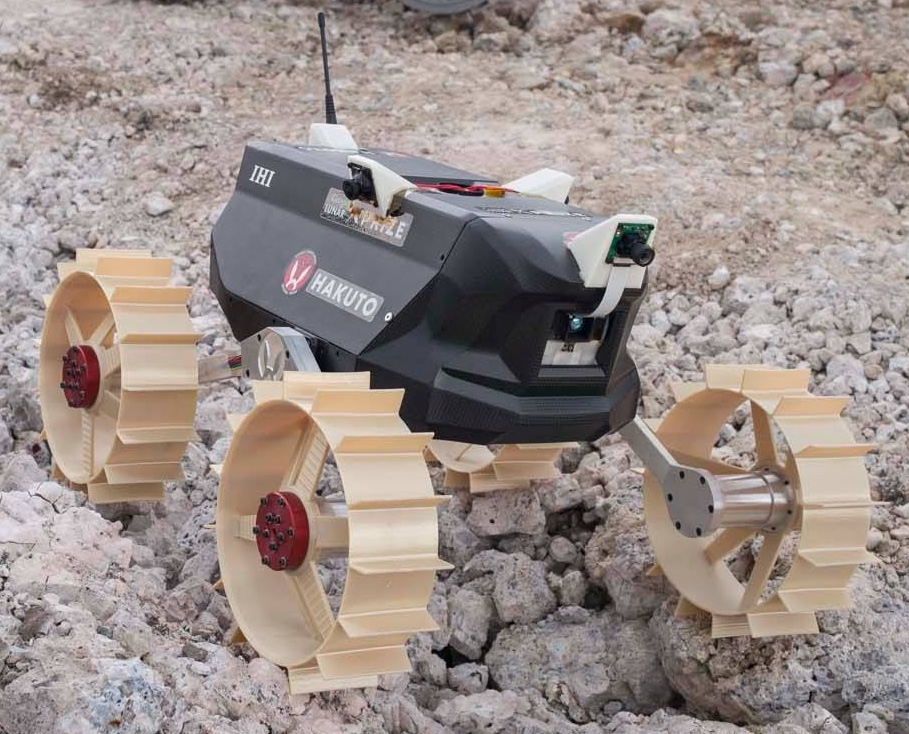
\includegraphics[width=\columnwidth]{images/moonraker.jpg}
    \caption{Hakuto's Moonraker ``Pre-Flight Model 2." Photo by George Thomas Mendel.}
    \label{fig:moonraker}
\end{figure}

\section{Ground Station Interface}

In early July 2015, Hakuto began designing a new ground station (GSN) software suite for the most recent version of the rover. Moonraker had been updated in several ways since the prior Pre-Flight Model, and many of its avionics, including its software, were updated and redesigned, breaking compatibility with the previous version of the ground station software. We worked together to evaluate the current and future needs of the rover, and to redesign and reimplement software to optimally fit these needs.

Our discussions focused on optimizing performance, reliability, and maintainability of the software. The latter factor was of particular concern, given that the software was to be used and maintained in a university laboratory environment, with many students---some of them inexperienced in software engineering---potentially responsible for updating the software and adding new features. After evaluating a list of disparate choices, including C++ on Linux with the Qt framework, and multi-platform JavaScript running in HTML5, we ultimately decided that the ideal choice would be the Unity Game Engine, for its high frequency of software updates, its active developer community, and its aerospace legacy within the NASA Jet Propulsion Laboratory \cite{jplunity}. 

\section{Rover Data Path}

In Hakuto's network configuration, Moonraker sends data packets over radio from the Moon, and they are intercepted on Earth and relayed to the ground station over the Internet. Subsequently, these packets are decoded and processed in order to be visualized by the ground station. The data is stored locally in memory by the ground station software for subsequent display. A flowchart of this data path is shown in Fig.~\ref{fig:data_path}.

\begin{figure}[h]
\centering
    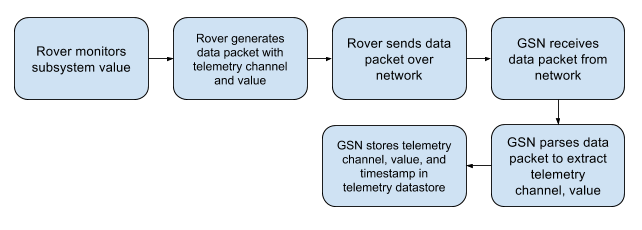
\includegraphics[width=\columnwidth]{images/rover_data_flow.png}
    \caption{Moonraker's communication flow, from rover subsystem to ground station data storage, is shown.}
    \label{fig:data_path}
\end{figure}

\subsection{Non-FDIR-Related Components}

The focus of this thesis is on the fault detective and correlative visualizations implemented within the ground station, so we will spend the bulk of the time focusing on these components. However, several non-FDIR-related components were implemented as well, briefly described below to provide context:

\begin{itemize}
    \item \textit{Numerical telemetry display}, to visually show the state of various sensors within subsystems (such as IMU accelerations, motor voltages, and board temperatures), as well as internal software metrics. Whenever possible, telemetry data was placed in semantically meaningful positions and groups, to improve discoverability.
    \item \textit{Attitude display and visual tachometer}, to provide more intuitive visualizations of pitch, roll, and current wheel rotation rate (which roughly corresponds to vehicle speed).
    \item \textit{Telemetry change indicators}, to point out data channels that have strong downward or upward trends over time.
    \item \textit{Quad-camera display}, to display the most recent images and streaming video from the rover cameras.
    \item \textit{Connectivity map}, to show the state of connectivity to various subsystems based on the elapsed time since packets from those subsystems have been received.
    \item \textit{Immersive viewing}, allowing users to view the camera data in an embedded 3D mapping.
    \item \textit{Map display}, showing the position of the rover with respect to the surrounding selenography, based on mobility subsystem and SLAM telemetry.
    \item \textit{Audio alarms}, to draw the user's attention to the UI in the event of faults.
    \item \textit{Telemetry saving, loading, and playback}, to facilitate the review of mission events after the fact.
\end{itemize}

\subsection{FDIR-Related Components}

In comparison with traditional aerospace ground station software, particular attention was given in this application to FDIR-related components. The components below were implemented and used extensively during normal operation.

\subsubsection{Threshold-based fault detection}

In order to build a threshold-based fault detection system for Moonraker, we worked with engineers on our team to define the ``danger" thresholds that indicated points of severe jeopardy, as well as the ``warning" thresholds that indicated points of concern. We implemented these thresholds in our ground station software as a general-purpose fault detection engine. Faults are detected constantly, and are displayed to the user via color and detailed information. All fault occurrence details and times are logged for future review as well. See Figure~\ref{fig:mobility_telem_subpanel}.

\begin{figure}[h]
\centering
    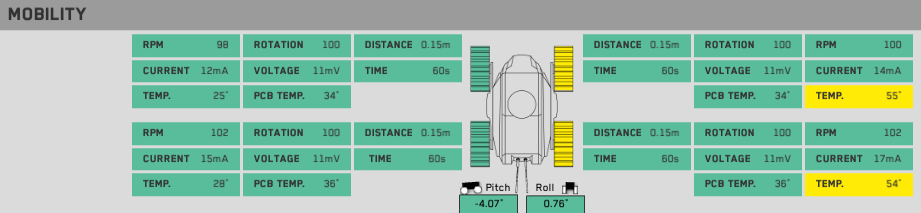
\includegraphics[width=\columnwidth]{images/mobility_telem_subpanel.png}
    \caption{Various telemetry values are shown for the mobility subsystem. Colors indicate current fault detection levels, with green representing a nominal state.}
    \label{fig:mobility_telem_subpanel}
\end{figure}

\subsubsection{Fault alert panel}

For safety, faults that have occurred need to be easily visible and understood by human operators. Towards this end, a highly visible, brightly colored alert panel was placed at the top of the screen seen by human operators. Each panel cell corresponds to a subsystem or other type of data grouping, and any issues with that grouping (i.e., faults that occur on monitored channels) will trigger a color change on that cell. Interacting with the cell can give the user more information on the fault (see the next section for details). See Figure~\ref{fig:alert_panel}.

\begin{figure}[h]
\centering
    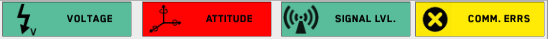
\includegraphics[width=\columnwidth]{images/alert_panel.png}
    \caption{An alert panel monitors potential faults on various different subsystems, indicating any faults and their severity by color.}
    \label{fig:alert_panel}
\end{figure}

\subsubsection{Expert fault information}

Ensuring human understanding of fault data is an essential part of the fault diagnosis and recovery process. As such, it's important to design a system where detailed information can be provided about individual faults that have occurred, while maintaining a high-level understanding of which systems are behaving anomalously. The system designed allows for this hierarchical organization of information. When high-level fault information is indicated in the ``fault alert panel," more concise information is provided in the ``fault information panel," including which anomalous data channels are contributing to the problem. The fault information is highly extensible, allowing for any other additional fault-related notes that system designers or operators would like to include for reference. This additional information, uncommon in traditional fault monitoring systems, accelerates the fault diagnosis problem by immediately pointing towards possible root causes. See Figure~\ref{fig:fault_info2}.

\begin{figure}[h]
\centering
    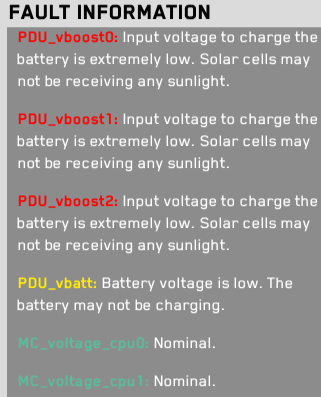
\includegraphics[width=0.4\columnwidth]{images/fault_info2.png}
    \caption{Information for monitored faults on a given subsystem.}
    \label{fig:fault_info2}
\end{figure}

\subsubsection{Correlative Functionality}

The Pearson Correlation Coefficient was chosen as an algorithm for calculating correlation between sets of data channels, in order to give a metric of their mutual ``connectedness." This algorithm was chosen for its simple and efficient calculations, under the (in retrospect, na\"{i}ve) assumption of linear relationships.

To visualize this data, a two-dimensional corrgram was used, visualizing relationships between data channels as a matrix with cell shadings representative of the PCC score of each relationship. The hue of each cell shows the sign of the correlation, and the intensity shows the strength of that correlation. This visualization allows an operator to see changing channel correlations, which may suggest possible interconnectedness or causation and aid with troubleshooting. See Figure~\ref{fig:corr_map}.

To clarify the flow of this data, pseudocode for the algorithm used is shown in Algorithm~\ref{alg:corrgram_get}. Assume that a pre-generated $n \times n$ grid of transparent blocks, $\textbf{Corr}$, is displayed on the screen. Also assume that $\textbf{GetColor}$ refers to an arbitrary function which maps from a PCC score $\in [-1,1]$ to an RGB color $(r, g, b) \in \mathbb{R}^{3}$, where $0 \leq r, g, b \leq 255$. We experimented with several variations of this function, and found that a linear mapping exaggerated the importance of low correlation scores, which led to the development of a hand-tuned exponential color mapping function to produce the correct scores. Certain work has explored the complexities of determining a proper mapping, which relate to the non-linearity of human perception of color \cite{friendly2002corrgrams}. Other work has suggested the efficacy of pre-squaring the PCC score before display, which instead results in displaying the coefficient of determination (i.e., the shared portion of the variance) for the pair of data items, which incidentally corresponds to a more intuitive human understanding of data connectivity \cite{rummelcorrelation}.

\begin{algorithm}
    \caption{Animated Corrgram Generation Algorithm}\label{alg:corrgram_get}
    \begin{algorithmic}[1]
        \Procedure{CorrgramGenerator}{$M$}\Comment{Takes data matrix $M \in \mathbb{R}^{n \times t}$.}
        \State $M_{r} \gets \{U_{:,j}\}_{j=t-s}^{n}$ \Comment{Reduce data to most recent $s$ points.}
        \State $C\gets \textbf{PCC}_{s}(M_{r})$ \Comment{Calculate a symmetric PCC matrix using last $s$ points.}
        \For{$\textbf{row} = 1~\textbf{to}~n$}
            \For{$\textbf{col} = 1~\textbf{to}~n$}
                \State $\textbf{color} = \textbf{GetColor}(C_{row, col})$ \Comment{Convert PCC score to a color.}
                \State $\textbf{Corr}_{row, col}\textbf{.color} \gets \textbf{color}$ \Comment{Assign color to cell in corrgram.}
            \EndFor
        \EndFor
        \EndProcedure \Comment{Algorithm is re-run on every graphical update.}
    \end{algorithmic}
\end{algorithm}

A few additional modifications were applied in order to make this algorithm performant. For instance, the entire corrgram is not updated at once, due to the performance hit from calculating new PCC scores for thousands of corrgram cells on each graphical update. Instead, a subset of the corrgram cells are updated, resulting in a ``rolling" effect wherein cells update gradually, with a full update of the corrgram being achieved on the order of once per second.

We also built functionality to adjust the sampling rate, the period of time over which samples are taken, and parameters related to averaging for smoothing out noise. Channel pairs may also be filtered via substring search, or via current fault states.

\begin{figure}[h]
\centering
    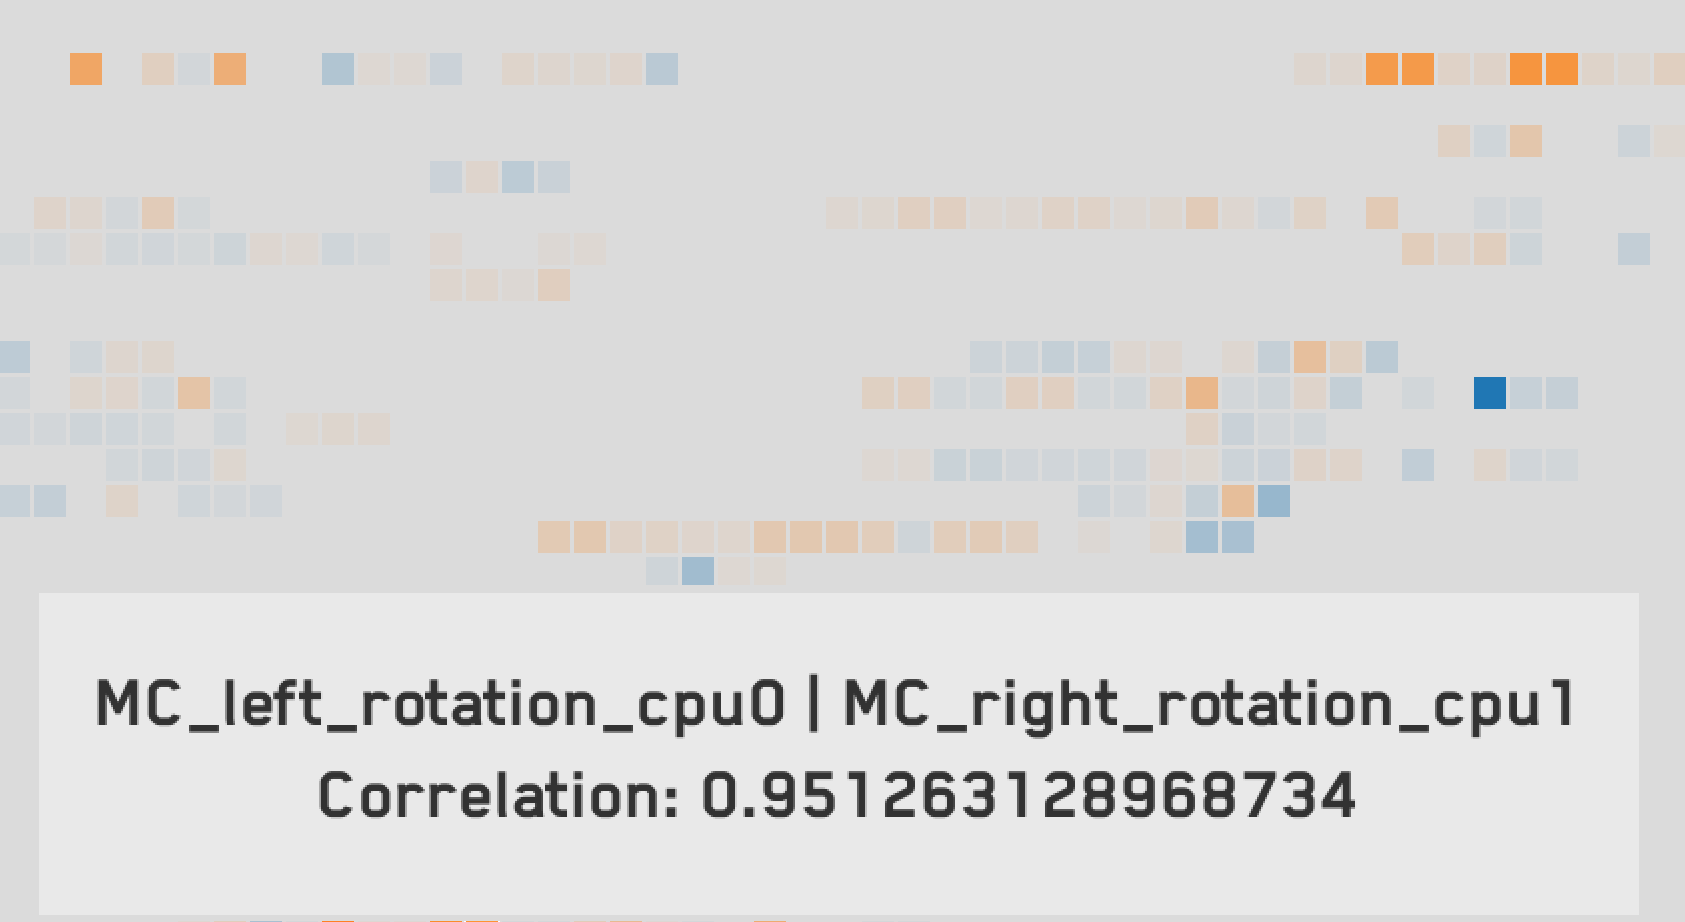
\includegraphics[width=\columnwidth]{images/corr_map.png}
    \caption{Correlation map visualization showing various different data channel pairs and their correlations. Bright orange signifies a high positive correlation, and bright blue is a high negative correlation.}
    \label{fig:corr_map}
\end{figure}

The next chapter will discuss testing we performed to validate the various components of this ground station interface.